% !Mode:: "TeX:UTF-8"
\documentclass[11pt]{book}

%\usepackage{lnote}

\usepackage{CJKutf8,CJKnumb}
%\usepackage{CJKpunct} %a homemade package

\usepackage{fancyhdr}
\usepackage{titlesec}

\usepackage{indentfirst}
\usepackage{paralist}
\usepackage{verbatim}

\usepackage[plain]{fancyref}
%%\usepackage[bookmarksnumbered,dvipdfmx,unicode, pdfborder=1,breaklinks,colorlinks,linkcolor=RoyalBlue3,urlcolor=blue]{hyperref}
\usepackage[bookmarksnumbered,unicode, pdfborder=1,breaklinks,colorlinks,linkcolor=RoyalBlue3,urlcolor=blue]{hyperref}
\usepackage{makeidx}

\usepackage{mflogo,texnames}
\usepackage{textcomp}

\usepackage{amsmath,amsfonts,amsthm}

\usepackage[x11names]{xcolor} %must before tikz, x11names defines RoyalBlue3
\usepackage{graphicx}
%\usepackage{ps4pdf} %conflict with tabularx
\usepackage{pstricks,pst-plot,pst-eps}
\usepackage{subfig}
\def\pgfsysdriver{pgfsys-dvipdfmx.def} %put before tikz
%%\usepackage{tikz}

\usepackage{booktabs,tabularx,multirow,colortbl,longtable}

\usepackage{chapterbib}
\usepackage[sectionbib,super,square,sort&compress]{natbib}


%中文设置
\newcommand{\song}{\CJKfamily{usong}}
\newcommand{\fang}{\CJKfamily{ufang}}
\newcommand{\kai}{\CJKfamily{ukai}}
\newcommand{\hei}{\CJKfamily{uhei}}

%\AtBeginDvi{\special{pdf:tounicode GBK-EUC-UCS2}} %not necessary if use UTF8.

%行距
\renewcommand{\baselinestretch}{1.25}

%页眉页脚
\pagestyle{fancy}
\fancyhf{}
\fancyhead[LE,RO]{\thepage}
\fancyhead[RE]{\leftmark}
\fancyhead[LO]{\rightmark}
\fancypagestyle{plain}{%设置plain页格式
    \fancyhf{}
    \renewcommand{\headrulewidth}{0pt}
}

%章节
\renewcommand{\chaptername}{第\CJKnumber{\thechapter}章}
\newcommand{\sectionname}{节}
\renewcommand{\figurename}{图}
\renewcommand{\tablename}{表}
\renewcommand{\bibname}{参考文献}
\renewcommand{\contentsname}{目~录}
\renewcommand{\listfigurename}{图~目~录}
\renewcommand{\listtablename}{表~目~录}
\renewcommand{\indexname}{索~引}
\titleformat{\chapter}[block]{\center\Huge}{\chaptername}{20pt}{}

\makeindex

%空白页
%%\makeatletter
\def\cleardoublepage{
    \clearpage\if@twoside\ifodd\c@page\else
    \hbox{}
    \vspace*{\fill}
    \begin{center}
        看什么看,没见过空白页?
    \end{center}
    \vspace{\fill}
    \thispagestyle{empty}
    \newpage
    \if@twocolumn\hbox{}\newpage\fi\fi\fi
}
\makeatother

%Code demo
%%\makeatletter
\newenvironment{mycode}{
    \noindent
    \newsavebox{\mybox}
    \begin{lrbox}{\mybox}
    \begin{minipage}[c]{.945\textwidth}
    \begin{verbatim}
}{
    \end{verbatim}
    \end{minipage}
    \end{lrbox}%
    \setlength{\fboxsep}{8pt}
    \colorbox{demo@bgcolor}{\usebox{\mybox}}
    \setlength{\fboxsep}{\oldfboxsep}
}

\newenvironment{myoutput}{
    \noindent
    \begin{lrbox}{\@tempboxa}
    \begin{minipage}[c]{.945\textwidth}
}{
    \end{minipage}
    \end{lrbox}%
    \setlength{\fboxsep}{8pt}
    \fbox{\usebox{\@tempboxa}}
    \setlength{\fboxsep}{\oldfboxsep}
}
\makeatother


\definecolor{demo@bgcolor}{gray}{.8}
\let\oldfboxsep\fboxsep
\newwrite\file
\newsavebox{\mybox}

\makeatletter
\def\demo@start{
    \begingroup% Lets Keep the Changes Local
    \@bsphack
    \immediate\openout \file \jobname.exa
    \let\do\@makeother\dospecials
    \catcode`\^^M\active
    \def\verbatim@processline{
        \immediate\write\file{\the\verbatim@line}
    }
    \verbatim@start
}

\def\demo@end{\immediate\closeout\file\@esphack\endgroup}

\def\demo@code#1#2{%
    \setlength{\fboxsep}{8pt}%
    \colorbox{#1}{%
    \begin{minipage}[c]{#2}
        \setlength{\fboxsep}{\oldfboxsep}
        \small\verbatiminput{\jobname.exa}
    \end{minipage}%
    }%
}

\def\demo@out#1{%
    \setlength{\fboxsep}{8pt}%
    \fbox{%
    \begin{minipage}[c]{#1}
        \setlength{\fboxsep}{\oldfboxsep}
        \small\input{\jobname.exa}
    \end{minipage}%
    }%
}

\newenvironment{code}{
    \demo@start
}{
    \demo@end
    \list{}{\itemindent-\leftmargin}
    \item
    \demo@code{demo@bgcolor}{.95\textwidth}
    \endlist
}

\newenvironment{halfcode}{
    \demo@start
}{
    \demo@end
    \list{}{\itemindent-\leftmargin}
    \item
    \demo@code{demo@bgcolor}{.52\textwidth}
    \endlist
}

\newenvironment{out}{
    \demo@start
}{
    \demo@end
    \list{}{\itemindent-\leftmargin}
    \item
    \demo@out{.95\textwidth}
    \endlist
}

\newenvironment{demo}{
    \demo@start
}{
    \demo@end
    \list{}{\itemindent-\leftmargin}
    \item
    \makebox[\textwidth][c]{%
        \demo@code{demo@bgcolor}{.52\textwidth}%
        \hspace{10pt}%
        \demo@out{.36\textwidth}%
    }
    \endlist
}

\newenvironment{fdemo}[1]{
    \begin{lrbox}{\mybox}%
    \setlength{\fboxsep}{8pt}%
    \fbox{%
    \begin{minipage}[c]{.36\textwidth}
        \setlength{\fboxsep}{\oldfboxsep}
        \small{#1}
    \end{minipage}%
    }%
    \end{lrbox}
    \demo@start
}{
    \demo@end
    \list{}{\itemindent-\leftmargin}
    \item
    \makebox[\textwidth][c]{%
        \demo@code{demo@bgcolor}{0.52\textwidth}%
        \hspace{10pt}%
        \usebox{\mybox}%
    }
    \endlist
}
\makeatother

\def\reflect#1{{\setbox0=\hbox{#1}\rlap{\kern0.5\wd0
  \special{x:gsave}\special{x:scale -1 1}}\box0 \special{x:grestore}}}
\def\XeTeX{\leavevmode
  \setbox0=\hbox{X\lower.5ex\hbox{\kern-.15em\reflect{E}}\kern-.1667em \TeX}%
  \dp0=0pt\ht0=0pt\box0 }

%图形设置
\DeclareGraphicsExtensions{.eps,.mps,.pdf,.jpg,.png}

%\usetikzlibrary{arrows,decorations,positioning}
%\pgfsetxvec{\pgfpoint{10pt}{0}}
%\pgfsetyvec{\pgfpoint{0}{10pt}}
%\tikzset{
%    box/.style={rectangle,rounded corners=6pt,
%        minimum width=40pt, minimum height=20pt, inner sep=6pt,
%        draw=gray,thick,fill=lightgray},
%    arrow/.style={->, shorten >=1pt, >=stealth', semithick},
%    larrow/.style={->, shorten >=1pt, >=stealth', semithick},
%    bloop/.style={semithick, to path={-- ++(0,-35pt) -| (\tikztotarget)}},
%    rloop/.style={semithick, to path={-- ++(10pt,0) |- (\tikztotarget)}}
%}

\graphicspath{{pictures/}}

\begin{document}
%\begin{CJK*}{UTF8}{usong}
\begin{CJK}{UTF8}{hei}
\CJKindent %can only be used in the CJK environment
\CJKtilde

\frontmatter

\title{\Huge arm汇编语言混合编程}
\author{zhangzhao\footnote{\href{mailto:mail.zhangzhao@gmail.com}{mailto:mail.zhangzhao@gmail.com}}}
\date{2011年11月15日}
\maketitle


%\setcitestyle{numbers,square}

%前言页眉
\renewcommand{\chaptermark}[1]{\markboth{#1}{}}

\include{preface}
\tableofcontents

\mainmatter
%正文页眉
\renewcommand{\chaptermark}[1]{\markboth{\chaptername\ #1}{}}
\renewcommand{\sectionmark}[1]{\markright{\thesection\ #1}}

\chapter{背景}

\begin{quotation}
满纸荒唐言,一把辛酸泪!都云作者痴,谁解其中味?\footnote{想法付诸实现并能拿得出手确实不容易。}
\begin{flushright}
--- 曹雪芹
\end{flushright}
\end{quotation}

为了更好地理解计算机体系结构,了解程序工作原理。
本文从汇编语言的角度来解释程序函数调用的过程。
汇编语言和C语言混合编程主要分为两种
\begin{itemize}
    \item C函数内部直接嵌套汇编语句
    \item 直接编写一个汇编函数供别人调用
\end{itemize}
本文主要讲述第二种中函数调用过程中ARM CPU的寄存器是如何
约定使用的
本文不讲一些形象的比喻,只是使用实际的代码
运行过程中的gdb跟踪的实例来讲解
本文只讲解用户模式和系统模式,不包括特权模式、中止模式
未定义命令模式、外部中断模式、快速中断模式

\chapter{关键字}

\begin{itemize}
    \item APCS ARM 过程调用标准(ARM  Procedure Call Standard)
    \item ASM  汇编语言(assembler)
    \item BackTrace 栈回溯,一般用于程序崩溃时回溯当前运行的栈
\end{itemize}
%\newpage

\chapter{前提}
\section{本文假设你已经有了...}
\subsection{硬件}
\begin{itemize}
    \item arm开发板一块,arm9以上
\end{itemize}
\subsection{软件}
\begin{itemize}
    \item GNU arm编译器一套
    \item 运行于开发板的uboot linux kernel rootfs一套
    \item vimgdb编辑器一套,vim加了gdb的patch以后我称之为vimgdb
    \item gdb\_mappings.vim 的vim插件,用来映射gdb快捷键
\end{itemize}

\section{本文假设你已经懂了...}
\begin{itemize}
    \item 良好的c语言基础
    \item 熟练的linux环境操作
    \item 熟练的gdb远程调试
    \item arm寄存器的名称、别名及其用途
    \item GNU AT\&T汇编的基本格式
    \item 少量的arm汇编知识
    \item 清晰的头脑
\end{itemize}

%\newpage

\chapter{系统配置}

\begin{quotation}
滚滚长江东逝水,浪花淘尽英雄。是非成败转头空。青山依旧在,几度夕阳红。

白发渔樵江渚上,惯看秋月春风。一壶浊酒喜相逢。古今多少事,都付笑谈中。
\begin{flushright}
---~杨慎《临江仙》
\end{flushright}
\end{quotation}

\section{helloworld}
直接上代码
\begin{code}
int fun1(int a, int b)
{
    int c;
    c = 10;
    return 0;
}
int main(int argc, char *argv[])
{
    int a;
    a = fun1(1, 2);
    return 0;
}
\end{code}
保存上述代码为helloworld\_c.c

\section{build}
编译代码并且拷贝到nfs中,以使arm板子能运行改程序
\begin{code}
arm-linux-gcc -g helloworld_c.c -o helloworld_c.arm
cp helloworld_c.arm destdir
\end{code}

\section{run}
使用gdbserver运行代码,客户端(PC)进行远程调试
arm板运行如下命令
\begin{code}
echo 0 > /proc/sys/kernel/randomize_va_space "调整每次程序启动为同一个栈起始地址,方便调试
gdbserver yourBoardIPAddress:888 helloworld_c.arm
\end{code}
pc运行如下命令
\begin{code}
vim helloworld_c.c "打开文件
F7 "映射vimgdb快捷键
file helloworld_c.arm "加载helloworld_c.arm文件符号
target remote yourBoardIPAddress:888 "开始远程调试
Ctrl+b "在helloworld_c.c下断点
Shift+c "continue运行
ni "进入汇编调试模式
si "汇编过程调用单步进入
\end{code}

\section{ASM}
\begin{code}
Dump of assembler code for function main:
0x00008454 <main+0>:	mov	r12, sp
0x00008458 <main+4>:	stmdb	sp!, {r11, r12, lr, pc}
0x0000845c <main+8>:	sub	r11, r12, #4	; 0x4
0x00008460 <main+12>:	sub	sp, sp, #12	; 0xc
0x00008464 <main+16>:	str	r0, [r11, #-16]
0x00008468 <main+20>:	str	r1, [r11, #-20]
0x0000846c <main+24>:	mov	r0, #1	; 0x1
0x00008470 <main+28>:	mov	r1, #2	; 0x2
0x00008474 <main+32>:	bl	0x8428 <fun1>
0x00008478 <main+36>:	str	r0, [r11, #-24]
0x0000847c <main+40>:	mov	r0, #0	; 0x0
0x00008480 <main+44>:	sub	sp, r11, #12	; 0xc
0x00008484 <main+48>:	ldmia	sp, {r11, sp, pc}
End of assembler dump.

Dump of assembler code for function fun1:
0x00008428 <fun1+0>:	mov	r12, sp
0x0000842c <fun1+4>:	stmdb	sp!, {r11, r12, lr, pc}
0x00008430 <fun1+8>:	sub	r11, r12, #4	; 0x4
0x00008434 <fun1+12>:	sub	sp, sp, #12	; 0xc
0x00008438 <fun1+16>:	str	r0, [r11, #-16]
0x0000843c <fun1+20>:	str	r1, [r11, #-20]
0x00008440 <fun1+24>:	mov	r3, #10	; 0xa
0x00008444 <fun1+28>:	str	r3, [r11, #-24]
0x00008448 <fun1+32>:	mov	r0, #0	; 0x0
0x0000844c <fun1+36>:	sub	sp, r11, #12	; 0xc
0x00008450 <fun1+40>:	ldmia	sp, {r11, sp, pc}
End of assembler dump.
\end{code}

\section{分析}
本文从代码段0x0000846c开始讲解
每张图都是在还没有执行该指令时读取并绘制的

\begin{figure}[htbp]%位置选项
\centering
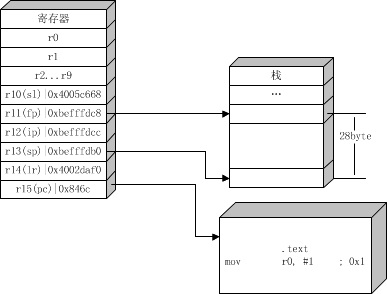
\includegraphics[bb=0 0 387 294,scale=0.7]{armapcs1_1.png}
\caption{准备压入func1参数的a}
\label{fig:anna}
\end{figure}

\begin{figure}[htbp]%位置选项
\centering
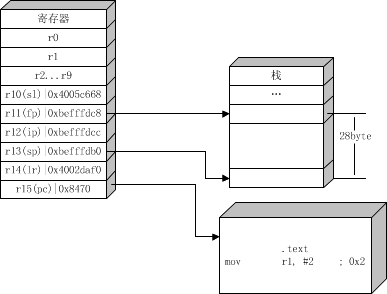
\includegraphics[bb=0 0 387 294,scale=0.7]{armapcs1_2.png}
\caption{已经压入func1参数的a 准备压入func1参数的b}
\label{fig:anna}
\end{figure}

\begin{figure}[htbp]%位置选项
\centering
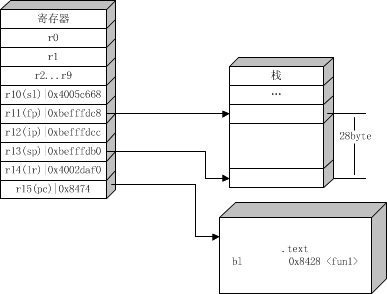
\includegraphics[bb=0 0 387 294,scale=0.7]{armapcs1_3.png}
\caption{已经压入func1参数的b 准备调用func1}
\label{fig:anna}
\end{figure}

\begin{figure}[htbp]%位置选项
\centering
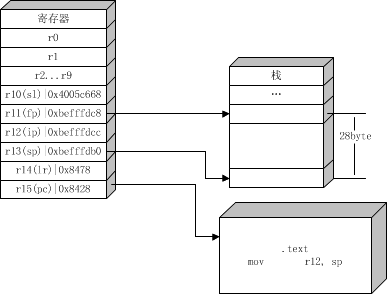
\includegraphics[bb=0 0 387 294,scale=0.7]{armapcs1_4.png}
\caption{转到func1代码段执行 准备将当前栈顶指针暂存入r12(ip),方便计算当前func1的fp指针}
\label{fig:anna}
\end{figure}

\begin{figure}[htbp]%位置选项
\centering
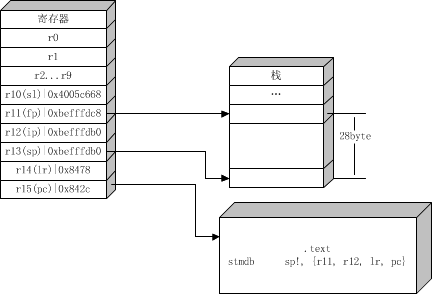
\includegraphics[bb=0 0 432 294,scale=0.7]{armapcs1_5.png}
\caption{当前栈顶指针暂存入r12(ip) ok, 准备存储当前的pc lr ip fp,以便函数返回时恢复上一个函数的寄存器}
\label{fig:anna}
\end{figure}

\begin{figure}[htbp]%位置选项
\centering
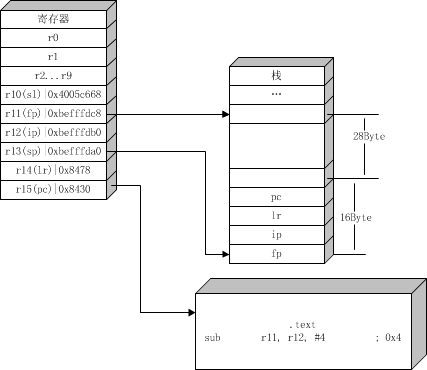
\includegraphics[bb=0 0 427 370,scale=0.7]{armapcs1_6.png}
\caption{存储当前的pc lr ip fp ok 上一个栈顶指针-4个字节就是当前的栈帧}
\label{fig:anna}
\end{figure}

\begin{figure}[htbp]%位置选项
\centering
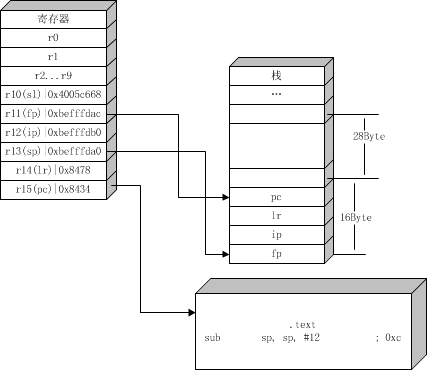
\includegraphics[bb=0 0 427 370,scale=0.7]{armapcs1_7.png}
\caption{当前栈帧计算ok 准备继续在栈上开辟12个字节的空间,方便存储本地自动变量}
\label{fig:anna}
\end{figure}


\begin{code}
存储第一个参数到当前sp之下
0x00008438 <fun1+16>:	str	r0, [r11, #-16]
存储第一个参数到当前sp-4之下
0x0000843c <fun1+20>:	str	r1, [r11, #-20]
存储立即数10到r3寄存器
0x00008440 <fun1+24>:	mov	r3, #10	; 0xa
存储第一个参数到当前sp-8之下
0x00008444 <fun1+28>:	str	r3, [r11, #-24]
存储立即数10到r0寄存器 用于返回值
0x00008448 <fun1+32>:	mov	r0, #0	; 0x0
\end{code}


\begin{figure}[htbp]%位置选项
\centering
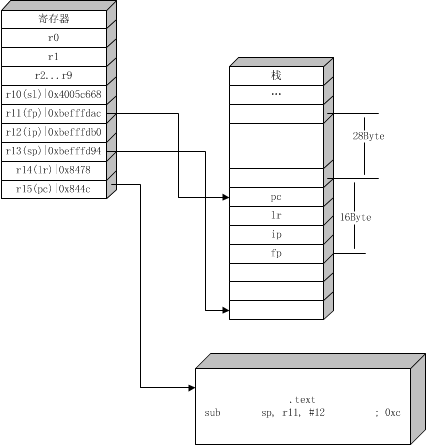
\includegraphics[bb=0 0 427 445,scale=0.7]{armapcs1_11.png}
\caption{当前返回值赋值给r0 ok 准备回退当前栈顶指针到func1栈顶-12处,以便读取内存中已经存储好的lr ip fp 到寄存器的pc sp r11}
\label{fig:anna}
\end{figure}

\begin{figure}[htbp]%位置选项
\centering
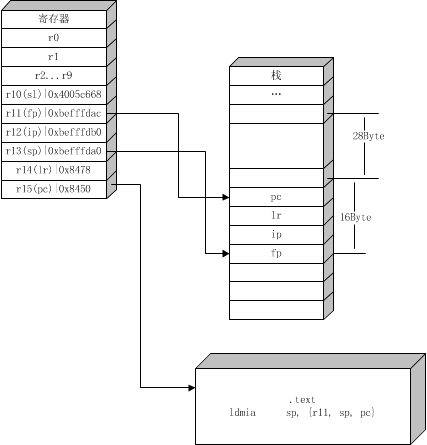
\includegraphics[bb=0 0 427 445,scale=0.7]{armapcs1_12.png}
\caption{回退当前栈顶指针到func1栈顶-12 ok,准备读取内存中已经存储好的lr ip fp 到寄存器的pc sp r11}
\label{fig:anna}
\end{figure}

\begin{figure}[htbp]%位置选项
\centering
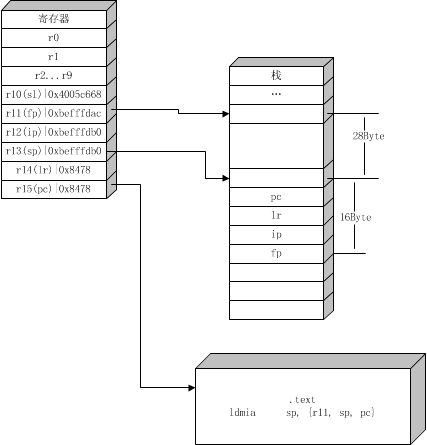
\includegraphics[bb=0 0 427 445,scale=0.7]{armapcs1_13.png}
\caption{读取内存中已经存储好的lr ip fp 到寄存器的pc sp r11 ok 函数回退完毕}
\label{fig:anna}
\end{figure}

%\newpage

\chapter{demo}

\newpage

\chapter{附录1}

\section{arm寄存器介绍}
\newpage
\begin{table}[htbp]
\caption{常用寄存器列表}
\centering
\begin{tabular}{p{20pt}p{20pt}p{20pt}p{100pt}}
    \toprule
    原名& 别名 & 又称 & 解释\\
    \midrule
    r0  &  a1 &      & \\
    r1  &  a2 &      & \\
    r2  &  a3 &      & \\
    r3  &  a4 &      & \\
    r4  &  v1 &      & \\
    r5  &  v2 &      & \\
    r6  &  v3 &      & \\
    r7  &  v4 &      & \\
    r8  &  v5 &      & \\
    r9  &  v6 &   sb & stack base\\
    r10 &  v7 &   sl & stack limit\\
    r11 &  v8 &   fp & frame pointer\\
    r12 &  ip &      & intra-procedure-call scratch register\\
    r13 &  sp &      & stack pointer\\
    r14 &  lr &      & link pointer\\
    r15 &  pc &      & program counter\\
    \bottomrule
\end{tabular}
\end{table}

\section{其他寄存器}

\subsection{Predeclared program status register names}
The following program status register names are predeclared:
\begin{itemize}
    \item cpsr and CPSR (current program status register)
    \item spsr and SPSR (saved program status register).
\end{itemize}

\subsection{Predeclared floating-point register names}
The following floating-point register names are predeclared:
\begin{itemize}
    \item f0-f7 and F0-F7 (FPA registers)
    \item s0-s31 and S0-S31 (VFP single-precision registers)
    \item d0-d15 and D0-D15 (VFP double-precision registers).
\end{itemize}

\subsection{Predeclared coprocessor names}
The following coprocessor names and coprocessor register names are predeclared:
\begin{itemize}
    \item p0-p15 (coprocessors 0-15)
    \item c0-c15 (coprocessor registers 0-15).
\end{itemize}



%\backmatter
%\include{postcript}

%\chapter*{索引}
%\printindex

\newpage

%\end{CJK*}
\end{CJK}

\end{document}
